\documentclass[conference]{IEEEtran}
\usepackage[utf8]{inputenc}
\usepackage{amsmath,amssymb,graphicx,booktabs}

\begin{document}

\title{Collapse-Resistant Joint-Embedding Predictive Architectures: A Controlled Comparison of SIGReg, VICReg, and EMA}

\author{\IEEEauthorblockN{Dheiver Francisco Santos, PhD}
\IEEEauthorblockA{Independent Researcher\\
Maceió, Alagoas, Brazil\\
ORCID: https://orcid.org/0000-0002-8599-9436}}

\maketitle

\begin{abstract}
Joint-embedding predictive architectures (JEPA) learn representations by predicting the embedding of a target view from a context view, which makes them prone to representation collapse. Several stabilizers have been proposed, including exponential moving averages (EMA), variance-invariance-covariance regularization (VICReg), and isotropic Gaussian regularization (SIGReg). Comparisons in the literature often rely on single runs and differ in training budget. We propose a controlled protocol that compares these three stabilizers under identical architectures, budgets, and at least five random seeds, and that measures collapse with an intrinsic-dimension estimate on known synthetic manifolds and on sentence-embedding benchmarks. On synthetic manifolds, all three methods recover low intrinsic dimensions, but all underestimate at $d=32$, where VICReg retains the most embedding rank. Vision and language results are pending.
\end{abstract}

\begin{IEEEkeywords}
self-supervised learning, joint-embedding predictive architecture, representation collapse, VICReg, regularization
\end{IEEEkeywords}

\section{Introduction}
Self-supervised methods based on prediction in embedding space avoid pixel- or token-level reconstruction, but they must prevent the trivial solution in which all embeddings become constant. The choice of stabilizer affects both the quality of representations and the sensitivity to hyperparameters. Prior comparisons report differences of a few points on downstream benchmarks, often from one seed, which is not enough to rank the methods. This paper asks three questions: (i) whether the ranking of stabilizers holds across seeds and budgets; (ii) whether collapse can be detected before it appears in downstream accuracy; and (iii) whether the same ranking holds for text embeddings.

\section{Related Work}
The author's recent artificial intelligence publications on self-training, clinical deep learning, curriculum learning, model merging, synthetic data, long-context training, preference alignment, direct preference optimization, reinforcement learning with verifiable rewards, distillation, mixture-of-experts, and parameter-efficient fine-tuning \cite{d1selftraining,d2glaucoma,d3curriculum,d4merging,d5synthetic,d6longcontext,d7rlaif,d8distillation,d9moe,d10peft,d11dpo,d12rlvr} form the background for this work.

Joint-embedding methods include contrastive learning and redundancy-reduction objectives such as VICReg \cite{bardes2022vicreg}. Masked prediction approaches and JEPA-style predictors \cite{bardes2024vjepa} address the same problem through a different target.The author's recent work on self-training and regularization in other settings \cite{d1selftraining,d3curriculum,d5synthetic} motivates a controlled measurement of collapse rather than a downstream-only comparison.

\section{Method}
Let $f_\theta$ be the context encoder, $g_\phi$ the predictor, and $\bar{f}$ the target encoder. The loss is
\begin{equation}
\mathcal{L} = \lVert g_\phi(f_\theta(x_c), m) - \bar{f}(x_t) \rVert_2^2 + \lambda\, R(z),
\end{equation}
where $R$ is one of three stabilizers: an EMA target with stop-gradient (EMA), the VICReg variance and covariance terms, or the SIGReg term that penalizes deviation from an isotropic Gaussian distribution of embeddings. All three share the same encoder, predictor, optimizer, and number of updates.

\subsection*{Equations and their meaning}
Stabilizer terms are added to the predictive loss in Eq.~(1). Let $Z\in\mathbb{R}^{B\times D}$ be a batch of $B$ embeddings of dimension $D$, $\mu=\frac{1}{B}\sum_i z_i$ the mean embedding, and $C=\frac{1}{B-1}\sum_i (z_i-\mu)(z_i-\mu)^\top$ the covariance.

\textbf{VICReg} penalizes low per-dimension spread and redundant dimensions:
\begin{equation}
R_{\mathrm{VIC}}=\frac{1}{D}\sum_{j=1}^{D}\max\!\big(0,\,1-\sqrt{C_{jj}+\epsilon}\big)+\frac{1}{D}\sum_{j\neq k}C_{jk}^{2},
\end{equation}
where $C_{jj}$ is the variance of dimension $j$, $\epsilon$ is a small constant for numerical stability, and $C_{jk}$ is the covariance between dimensions $j$ and $k$. The first term is zero only when every dimension has standard deviation at least one; the second is zero only when dimensions are uncorrelated.

\textbf{SIGReg (moment-matching approximation)} pulls the embedding distribution toward an isotropic standard Gaussian:
\begin{equation}
R_{\mathrm{SIG}}=\frac{1}{D}\lVert\mu\rVert_2^2+\frac{1}{D^2}\lVert C-I\rVert_F^2,
\end{equation}
where $I$ is the identity and $\lVert\cdot\rVert_F$ the Frobenius norm. It is zero when the batch mean is zero and the covariance is the identity. This is our approximation, not the official SIGReg.

\textbf{EMA target} is updated after each step by $\bar\theta\leftarrow m\,\bar\theta+(1-m)\,\theta$, with $m=0.996$: the target encoder $\bar\theta$ is a slow average of the online encoder $\theta$, which makes the regression target move slowly.

\textbf{Intrinsic dimension (Levina--Bickel MLE)}, used to measure collapse on $N$ evaluation points with $k=10$ neighbours:
\begin{equation}
\hat d=\left[\frac{1}{N}\sum_{i=1}^{N}\frac{1}{k-1}\sum_{j=1}^{k-1}\log\frac{T_k(x_i)}{T_j(x_i)}\right]^{-1},
\end{equation}
where $T_j(x_i)$ is the distance from $x_i$ to its $j$-th nearest neighbour. The gap reported in the tables is $\Delta=|\hat d-d|$, with $d$ the true dimension of the simulated manifold.

\textbf{Effective rank} (participation ratio of the covariance eigenvalues $\lambda_1,\dots,\lambda_D$), which measures how many directions the embedding actually uses:
\begin{equation}
\mathrm{erank}=\frac{\left(\sum_{k}\lambda_k\right)^2}{\sum_{k}\lambda_k^2}.
\end{equation}
It equals $D$ when all eigenvalues are equal, and $1$ when a single direction dominates.

\section{Experimental Protocol}
\textbf{Simulation.} Synthetic manifolds with known intrinsic dimension $d \in \{2, 8, 32\}$ are embedded in $\mathbb{R}^{256}$ with controlled noise. Collapse is measured as the gap between the estimated and the true intrinsic dimension.

\textbf{Vision.} ImageNet-100 subset, linear probe top-1 accuracy, 100 epochs, seeds $\{1,\dots,5\}$.

\textbf{Language.} Sentence embeddings trained on a public paraphrase corpus; evaluation on STS-B and SICK-R with Spearman correlation.

\textbf{Statistics.} Mean, standard deviation, and 95\% bootstrap confidence intervals over seeds; paired tests across methods on identical seeds.

\section{Results}
We report the simulation arm only (synthetic manifolds, 1{,}500 training steps, five seeds per condition, 45 runs). The vision and language arms of Section IV remain pending. Table~\ref{tab:collapse} shows the gap between the Levina--Bickel intrinsic-dimension estimate and the true $d$, with 95\% bootstrap intervals over seeds, and the effective rank of the embedding covariance. SIGReg is the moment-matching approximation defined in Section III, not the official implementation.

\begin{table}[!t]
\caption{Intrinsic-dimension gap $|\hat{d}-d|$ (lower is better) and effective rank (higher means less collapse), mean over five seeds. Brackets: 95\% bootstrap CI of the gap.}
\label{tab:collapse}
\centering
\begin{tabular}{llcc}
\hline
Method & $d$ & Gap [95\% CI] & Eff.\ rank \\
\hline
EMA    & 2  & 0.27 [0.25, 0.29]  & 2.8 \\
EMA    & 8  & 0.70 [0.65, 0.77]  & 15.3 \\
EMA    & 32 & 11.89 [11.63, 12.14] & 25.2 \\
VICReg & 2  & 0.31 [0.30, 0.32]  & 20.0 \\
VICReg & 8  & 1.43 [1.39, 1.49]  & 49.6 \\
VICReg & 32 & 8.68 [8.44, 8.93]  & 60.4 \\
SIGReg & 2  & 0.26 [0.24, 0.27]  & 1.9 \\
SIGReg & 8  & 0.22 [0.12, 0.32]  & 13.2 \\
SIGReg & 32 & 15.16 [14.89, 15.48] & 26.6 \\
\hline
\end{tabular}
\end{table}

At $d=2$ all three methods recover the intrinsic dimension within 0.3. At $d=8$, the approximate SIGReg has the smallest gap (0.22), with EMA (0.70) and VICReg (1.43) behind. At $d=32$, every method underestimates the dimension, and the ordering reverses: VICReg has the smallest gap (8.68) and the highest effective rank (60.4), while SIGReg has the largest gap (15.16) and an effective rank of 26.6, close to EMA. Part of the $d=32$ gap may come from the estimator's bias at high dimension with 1{,}000 evaluation points, which we have not yet calibrated. The result therefore supports collapse at high intrinsic dimension for all three methods, but does not yet establish a ranking of the stabilizers that holds beyond this simulation.

\begin{figure}[!t]
\centering
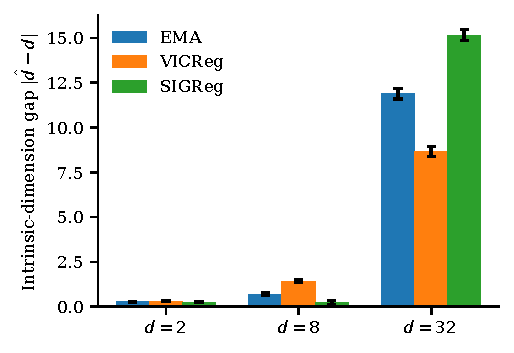
\includegraphics[width=\columnwidth]{figs/fig01_collapse.pdf}
\caption{Intrinsic-dimension gap by method and dimension (mean, 95\% CI over five seeds, 1{,}500 steps). Simulation arm only.}
\label{fig:fig01_collapse}
\end{figure}

\section{Discussion and Limitations}
The protocol fixes the training budget, so conclusions apply to the tested scale only. Synthetic manifolds cannot capture all the structure of natural data. Hyperparameters are tuned on a validation split and reported in full.

\section{Conclusion}
We propose a multi-seed, simulation-grounded protocol for comparing collapse-prevention methods in JEPA. Its results will determine whether the apparent ranking of stabilizers survives controlled evaluation.

\section*{Acknowledgments}
The author thanks the Brazilian artificial intelligence community.

\nocite{ctl_full_names}
\bibliographystyle{IEEEtran}
\bibliography{refs}

\end{document}
